\documentclass[11pt]{article}
\usepackage[T1]{fontenc}
\usepackage[utf8]{inputenc}
\usepackage{times}
\usepackage{inconsolata}
\usepackage{amsmath}
\usepackage{framed}
\usepackage{graphicx}
\usepackage{hyperref}
\hypersetup{colorlinks=true, linkcolor=blue, urlcolor=blue}
\usepackage{fancyvrb}
\usepackage[english]{babel}
\usepackage{enumitem} 
\setlist[itemize]{noitemsep}
\title{{\bf LAB 1:\\Requirements Modeling}\\ Preparations and instructions}
\author{Björn Regnell}
\date{\today}
\begin{document}
\maketitle

\section{Introduction}

\subsection{Purpose} This document provides instructions on how to prepare for and run a computer lab session on requirements modeling. The lab session illustrates how computer-supported requirements modeling can help in requirements engineering. {\it The preparations in Section~\ref{section:prep} should be completed before the actual lab is run.}

\subsection{Background} In this lab you will learn how to get started with requirements modeling through the open source tool \href{http://reqT.org}{reqT.org}, and reflect on how you could model requirements in your own project. The reqT tool enables scalable requirements modeling, ranging from small models of a couple of features to large models containing elaborate structures of thousands of requirements. 

Requirements engineering is a dynamic process where the understanding of an imagined future system (of systems) is evolving over time. During this evolution we can capture the knowledge and creative ideas that we elicit in various ways, depending on how we foresee the (later) usage of that knowledge. For example, we could create and use spread sheets, post-it notes, emails, wikis, video clips, mockups, sketches, diagrams, mathematical specifications, etc. If we want to keep track of many different types of inter-related requirements and if we see a future benefit of more structure beyond just a flat list, one option is to use requirements models where requirements-related information is expressed using relevant {\bf entity}, {\bf attribute}, and {\bf relation} concepts to capture what we want to model, as illustrated by this lab and the metamodel of reqT. 

\clearpage\newpage
\section{Preparations}\label{section:prep}

\begin{framed} \noindent Before doing the lab session in Section~\ref{section:instr}, complete all preparations 1--4 below and bring requested items to the lab. In particular you need to make sure that you can access the text files you prepare below at your lab session computer.
\end{framed}

\begin{enumerate}
\item {\bf Do the reqT "hello world".} Run the reqT hello world example on your computer, as explained here: \newline \url{http://reqt.org/documentation.html\#hello}
\item {\bf Draw a context diagram.} Draw a context diagram\footnote{\url{http://en.wikipedia.org/wiki/System_context_diagram}} that  is relevant to your development project. Make the drawing on paper and bring to the lab. The context diagram should include entities outside of the system you are building that communicate with your system. 
\item {\bf Create a context model.} Transform your context diagram into a reqT model, analogous to this  example: 
{\footnotesize\begin{verbatim}
Model(
  Product("hotelApp") interactsWith (
    User("receptionist"), 
    User("guest"), 
    System("telephony"), 
    System("accounting")))
\end{verbatim}}
Enter the code in your favorite editor and save it\footnote{If you prepare your files on mac/windows and use them on linux then reqT may provide strange results for some characters. See \url{http://manpages.ubuntu.com/manpages/maverick/man1/dos2unix.1.html}} in a text file called \verb+context.scala+
\item {\bf Create a list of features.} Make a list of at least 5 features relevant to your project, divided into named sections, analogous to the example below. Use the exact formatting and indentation according to the example with hash tag before the name of each section and an asterisk before the name of each feature: 
{\scriptsize\begin{verbatim}
# receptionFeatures
  * groupCheckIn
    Check in many guests arriving in bulk.
# adminFeatures
  * roomForecast
    Calculate room allocation prediction.
  * exportAccounting
    Export accounting data to external system.
\end{verbatim}}
Save the list of features in a text file called \verb+feat.txt+  
\end{enumerate}
\clearpage\newpage

\section{Lab instructions}\label{section:instr}

\subsection{Start reqT}
Download the reqT.jar file from \url{http://reqT.org} and start reqT in a terminal window using this command: \verb+java -jar reqT.jar+ as shown in Figure~\ref{fig:console}. Make sure you have the text files from your preparations from Section~\ref{section:prep} available in the same directory as you start reqT.

\begin{figure}[h]
    \centering
    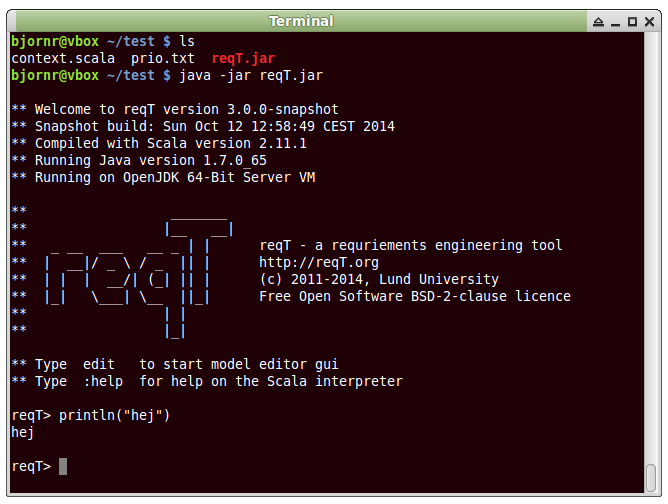
\includegraphics[width=0.7\textwidth]{console.png}
    \caption{The reqT console output after starting reqT in a terminal window.}
    \label{fig:console}
\end{figure}

In the reqT console these keystrokes and commands work as follows:
{\footnotesize 
\begin{itemize}[label={}]
\item <Ctrl+A> to move the cursor to the beginning of a line.
\item <Ctrl+E> to move the cursor to the end of a line.
\item <Ctrl+K> ''kill'': clears text after the cursor.
\item <Arrow Left/Right> to move the cursor backward/forward within a line. 
\item <Arrow Up/Down> to move backward/forward in the command history. 
\item <TAB> to invoke code completion.
\item \verb+:q+ to quit reqT when all threads and windows have been exited.
\item \verb+:help+ to get help on console commands.
\item \verb+sys.exit+ to exit reqT and kill all threads and any windows without saving.
\end{itemize}
}

{\begin{framed}\noindent
Try out the commands above in the reqT console. Use the \verb+:help+ command to figure out how to enter paste mode. Paste some text when in paste mode using mouse right-click. End paste mode pressing <ENTER> and then press <Ctrl+D> at the beginning of a new line. %What is the shortest, unambiguous abbreviation of the enter-paste-mode-command?  \underline{\hspace{2cm}}
\end{framed}}

\subsection{Create and update models using the reqT console}

\begin{framed}\noindent
Type in the following lines in the reqT console after the \verb+reqT>+ prompt. Press enter after each line. The \verb?+? operator is used to add elements to a model, and the  \verb?++? operator is used to append one model to another.

{\small\begin{verbatim}
reqT> val m1 = Model(Req("a") has Spec("sss"))

reqT> val m2 = m1 + (Req("b") has Prio(2))

reqT> val m3 = Model(Stakeholder("x") requires Req("a"))

reqT> ((m3 + Stakeholder("y")) ++ m2).size
\end{verbatim}}


\noindent What is the integer value result of the last evaluation above? Why?
\newline 
\newline
\newline \underline{\hspace{10cm}}

\vspace{7mm}
\noindent Continue to type in the following lines in the reqT console after the \verb+reqT>+ prompt. Press enter after each line. The \verb+for+ keyword is used to make a for-loop. The \verb+yield+ keyword is used in a for-comprehension to construct a sequence of values.  The \verb+val+ keyword is used to declare a name that refers to an immutable value (a constant) and the \verb+var+ keyword is used to declare a name that refers to a mutable value (a variable). The \verb?-? operator is used to remove elements from a model. With the \verb+transform+ method you can make transformations of specific elements in a model. 


{\scriptsize\begin{verbatim}
reqT> var m4 = (for (i <- 1 to 10) yield Req("r"+i)).toModel

reqT> (1 to 10).map(i => Req("r"+i)).toModel //alternative to above

reqT> m4 = Model(Stakeholder("x") requires m4)

reqT> m4 = m4 - Req("r7")

reqT> m4 -=  Req("r3")

reqT> m4.pp   //pretty-print m4

reqT> m4 = m4.transform{case Req(id) => Feature(id) has Status(ELICITED)}
\end{verbatim}}
\end{framed}
\begin{framed}\noindent
What is the size of the m4 model after the above transform? Why?
\newline
\verb+m4.size+
\newline
\newline \underline{\hspace{10cm}}
\end{framed}

\subsection{Investigate the reqT metamodel}

A reqT model can be viewed as a vector of elements. Elements can be entities, attributes and relations. An entity has an id of type String. An attribute holds a value that can be of different types. A relation connects and entity via a link of a certain RelationType to a submodel that, in turn, can contain elements. A part of the reqT metamodel is shown in Figure~\ref{fig:metamodel}. 

\begin{figure}[h]
    \centering
    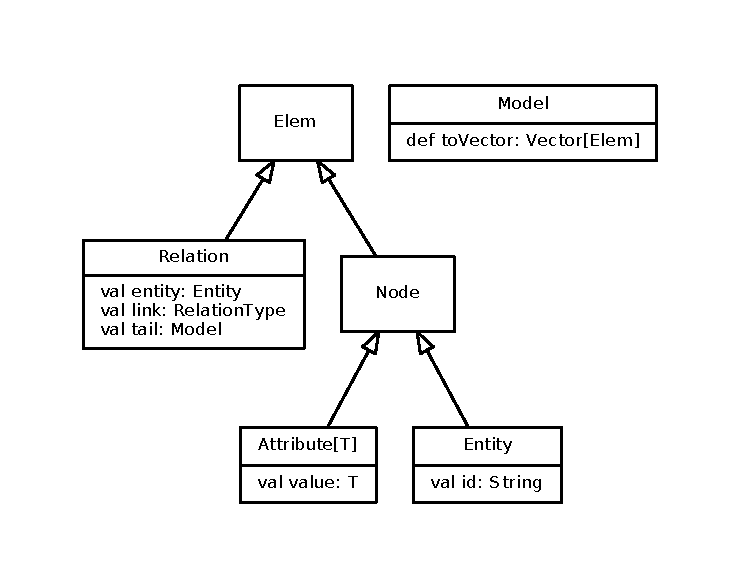
\includegraphics[width=\textwidth]{metamodel-simple.pdf}
    \caption{Some classes in the reqT metamodel.}
    \label{fig:metamodel}
\end{figure}

Investigate what different entity types, attribute types and relation types that the reqT metamodel contains, using the evaluations in the reqT console below. 

\begin{framed}{\footnotesize\begin{verbatim}
reqT> reqT.metamodel.  // Press <TAB> after the dot

reqT> reqT.metamodel.ent // Press <TAB> after the t

reqT> reqT.metamodel.entityTypes

reqT> reqT.metamodel.entityTypes.size

reqT> reqT.meta.model.pp

reqT> reqT.meta.model.collect{case Meta(_) => 1}.sum
\end{verbatim}}
\noindent The collect method gathers selected parts of a model into a vector. In the last evaluation above we collected the integer 1 for each occurrence of a Meta entity and sum all ones.
\newline\newline 
\noindent
How many different entity types, attribute types and relation types are there respectively in the reqT metamodel? 
\newline
\newline \underline{\hspace{10cm}}
\newline\newline
How many entity concepts of type \verb+Meta+  are there in the reqT metamodel (as calculated by the last evaluation above)? 
\newline
\newline \underline{\hspace{10cm}}
\end{framed}

The meta model elements can be used in many different ways. There are no restrictions on how to combine the elements, except for these three basic rules:
\begin{enumerate}[nolistsep]
\item {\bf Attribute identity}. A model or submodel can only contain at most {\it one} attribute of a specific type at its top level. However, the same type of attribute can co-exist if they reside in different submodels of the same model. 
\item {\bf Entity-Link identity}. A model or a submodel can only contain at most {\it one} entity with a certain id and a certain relation link at its top level. If you add an entity with the same id and the same relation link at the top level of a model or submodel, it will merge the elements of each submodel, and if the above rule applies then the last same-typed attribute will be overwrite the former. 
\item {\bf Leaf entity has empty submodel}. The \verb+has+-relation is special, as a leaf entity that has no relations to any subelements is equivalent to an entity with a has-relation to an empty submodel. 
\end{enumerate}

\begin{framed}\noindent
Try the subsequent statements in the reqT console, where \verb+Prio+ is an attribute type and \verb+Req+ is an entity type and \verb+has+ and \verb+requires+ are relation types. Make sure you can explain the evaluation results in relation to the rules above. Write the number of the rule(s) (1 -- 3) that is/are in effect besides each evaluation. 

{\scriptsize \begin{verbatim}
reqT> Model(Prio(1), Prio(2))

reqT> Model(Req("x") has (Prio(1), Prio(2)))

reqT> Model(Req("x") has Prio(1), Req("y") has Prio(1))

reqT> val m6 = Model(Req("x") has (Req("sub1"), Prio(1), Prio(2))) 

reqT> m6 + (Req("x") has (Req("sub2"),Prio(3)))

reqT> Model(Req("x") has ())

reqT> Model(Req("x") has Prio(1), Req("y") requires Prio(1)) - Prio(1)
\end{verbatim}}
\end{framed}

\begin{framed}\noindent
Create a model with two stakeholders \verb+a+ and \verb+b+, both requiring the same two features \verb+x+ and \verb+y+. The stakeholders' features shall have different priorities: a thinks x is of higher priority than y, while b thinks the opposite. Declare a constant called \verb+prio+ that refers to the model. Write the reqT code that describes your model below and then test it in the reqT console.
\newline
\newline 
\vspace{3cm}

\end{framed}

When you create a reqT model, you actually create an immutable, tree-like data structure that consists of computational objects in the Java Virtual Machine (JVM) runtime environment. When you encode reqT models you are actually coding in the \href{http://en.wikipedia.org/wiki/Scala_\%28programming_language\%29} {Scala programming language} that compiles to JVM byte code. The reqT metamodel classes are actually Scala classes and the reqT language is embedded in Scala. The \verb+reqT.jar+ file includes the Scala compiler and the reqT console wraps the so called Scala Read-Evaluate-Print-Loop (REPL), which enables any Scala code snippet to be interactively compiled and run on a line-by-line basis at the reqT prompt. 
\begin{framed}\noindent All the avaliable JDK classes can be accessed from the \verb+reqT>+ prompt. Try:
{\footnotesize\begin{verbatim}
javax.swing.JOptionPane.showMessageDialog(null,"Hello Swing!")
\end{verbatim}}
\end{framed}
\subsection{Access elements in models using paths}

A model is represented using a recursive data structure where relation elements can include submodels, which in turn can include relation elements that include submodels. The recursive nature of the model data structure thus enables hierarchical, tree-like requirements models of arbitrary depths. The submodels and elements of submodels at different levels can be accesses using paths that are constructed using the \verb+/+ operator called {\it enter}. 

A {\it head} is a start of a relation that combines an entity with a relation type using dot notation, such as  
\verb+Feature("x").has+ and \verb+Stakeholder("b").requires+  

Paths begin with a sequence of {\it heads} separated by \verb+/+ and may end with either (1) a head, (2) an entity, (3) an attribute type or (4) an attribute. The \verb+has+ relation is special: in paths an entity without any relation type is interpreted as an entity with a \verb+has+ relation. 

\begin{framed}\noindent
Try these path examples in the reqT console: 
{\scriptsize \begin{verbatim}
reqT> val p1 = Stakeholder("a").requires/Feature("x").has/Prio(42)

reqT> p1.depth    //write down the depth: _______

reqT> val p2 = Stakeholder("b")/Feature("x")/Prio(21)

reqT> p2.init

reqT> val p3 = p2.init/Feature("sub")/Prio(9)

reqT> p3.toModel

reqT> var pm = Vector(p1,p2,p3).toModel

reqT> pm/Stakeholder("b").has

reqT> pm/Stakeholder("b")

reqT> pm/Stakeholder("a").requires/Feature("x")/Prio

reqT> pm = pm + Stakeholder("a").requires/Feature("x")/Prio(1)

reqT> pm.leafPaths

reqT> pm.leafPaths.map(_.depth).max   //write down the max depth: ______
\end{verbatim}}
\end{framed}
\begin{framed}\noindent
Create a random model using the commands below, and write down its max depth: \underline{\hspace{1cm}}
{\scriptsize \begin{verbatim}
reqT> val rm = rndModel(10)
 
reqT> rm.pp

reqT> rm.leafPaths.map(_.depth).max    // Write down the max depth: _____

reqT> rm.leafPaths.filter(_.depth == 2).head
\end{verbatim}}
\noindent Write down the path to the first attribute at level 2:\newline\newline
\underline{\hspace{11cm}}
\end{framed}
 
If a path ends with an attribute type, then it refers to the corresponding value that is boxed by that attribute in a model. If the attribute is not available when the path is applied to a model with the enter operator \verb+/+ then a default value is produced. 

If you want to check the absence or presence of a value you can use the \verb+get+ method on a model. The \verb+get+ method takes a path as parameter and returns a value boxed in an instance of the \verb+Option+ class; if there was, e.g.,  an integer value of 42 then the option class evaluates to \verb+Some(42)+ or if there is no value then it evaluates to \verb+None+. You can get the actual value of an \verb+Option+ instance by calling the get method.    

\begin{framed}\noindent
Try these attribute type path examples in the reqT console: 
{\scriptsize \begin{verbatim}
reqT> val m = Model(Req("x") has Prio(1), Req("y"))

reqT> m / Req("x") / Prio

reqT> m / Req("y") / Prio    //write the default Prio value here _____

reqT> m.get(Req("x")/Prio)

reqT> (m/Req("x")).get(Prio).get    //same effect as previous    

reqT> m / Req("x") get Prio    //equivalent to previous

reqT> m / Req("x") get Prio get    

reqT> m / Req("y") get Prio get    
\end{verbatim}}
\noindent What happens if you try to call the \verb+get+ method on a non-existing value, as in the previous evaluation?
\newline\newline\underline{\hspace{10cm}}
\end{framed}

\subsection{Load and save files from the reqT console}

You can load text files into strings and save strings into text files using commands similar to: 
\begin{verbatim}
val s = load("myFile.txt")
"my String".save("myStringFile.txt")
\end{verbatim}
The \verb+ls+ command prints a list of files in the working directory. The \verb+pwd+ command prints the path of the working directory. The \verb+mkdir("tmp")+ command creates a new directory called \verb+tmp+ and \verb+cd("tmp")+ changes working directory to the directory \verb+tmp+ if it exists.

You can also serialize a model to a binary file, which for large files may take less space compared to a text file and it may also be quicker to save and load a large binary model to and from disk compared to a text model. To serialize a binary model to disk, just call the save method on a model. To load a binary model from disk use the \verb+Model.load("filename.reqt")+ command. It is recommend to use the file suffix \verb+.reqt+ to show that it is a serialized binary file.

\begin{framed}\noindent
Check that you have the files from the lab preparations in your working directory and load your context model and convert it to a reqT model from a string using the following evaluations: 
{\scriptsize \begin{verbatim}
reqT> ls
context.scala
prio.txt

reqT> var m = load("context.scala").toModel

reqT> m = Model(Title("My Cool Product"), Section("Context") has m)

reqT> m.toString.save("context-v2.scala")
Saved string to file: C:/Users/bjornr/tmp/context-v2.scala

reqT> m.save("context.reqt")
Model serialized to file: context.reqt
\end{verbatim}}
\noindent Create a large random model using the command: \newline{\scriptsize\verb+val r = rndModel(52,2)  //max 52 at top level and then max 26 etc.+} \newline and compare the binary model size on disk with the string model text file size, by checking the file sizes in your OS. If the files get so big that it takes too much time, reduce the number of max elements at top level.\newline
\newline Number of elements in the model: {\footnotesize\verb+r.size+} \underline{\hspace{2cm}} 
\newline Size of binary file: {\footnotesize\verb+r.save("big.reqt")+}  \underline{\hspace{2cm}} 
\newline Size of text file: {\footnotesize\verb+r.toString.save("big.scala")+} \underline{\hspace{2cm}}
\end{framed}

\subsection{Edit requirements with the reqT ModelTreeEditor GUI}

The reqT ModelTreeEditor is a graphical user interface for navigating and updating reqT model. You start the editor with the \verb+edit+ command. You can start many ModelTreeEditor windows. 

You can also preload a ModelTreeEditor instance with a model, e.g. called \verb+m+, by simply passing it as a paramter to the edit command, e.g. \verb+edit(m)+. The ModelTreeEditor is shown in Figure~\ref{fig:gui}. You can start many ModelTreeEditor windows by repeating the edit command.

\begin{figure}[h]
    \centering
    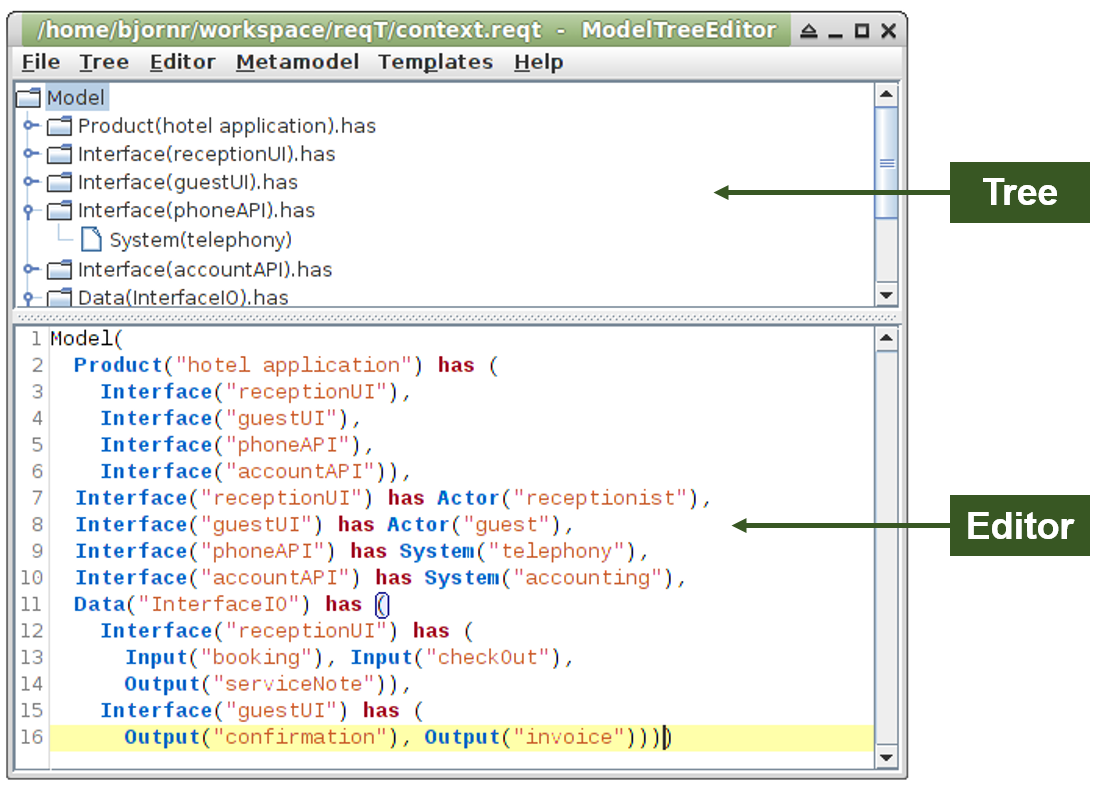
\includegraphics[width=0.95\textwidth]{gui.png}
    \caption{The reqT ModelTreeEditor graphical user interface.}
    \label{fig:gui}
\end{figure}

The reqT ModelTreeEditor gui has two parts:
\begin{itemize}
\item {\bf The Tree}. The Tree displays a tree view of a model, where each head node can be collapsed or expanded using the right and left arrows or by clicking on the handle by the left of the folder symbol. Model elements can be deleted using the forward DELETE key.
\item {\bf The Editor}. The Editor is aware of the reqT metamodel and Scala syntax and provides syntax coloring and code completion on model elements. Entities are of light blue color, relations are of red color and attributes are shown in green color. Reserved words of Scala are given a dark blue color.
\end{itemize}

The Tree and the Editor are two separate buffers, each having its own data. The Tree has its own reqT model converted to a javax.swing.JTree, while the content in the Editor can be any text (typically users have a textual representation of a reqT (sub)model undergoing  some update). 

By using the menu items in the Tree menu and the Editor menu you can transfer data from the Tree to the Editor and vice versa. You can also execute Scala code in the Editor by entering code in the Editor to the console for evaluation. The ModelTreeEditor has a number of convenient shortcuts to enable power users to quickly operate the Tree and Editor in concert.

\begin{framed}
Carry out these steps using the ModelTree Editor:
\begin{enumerate}
\item Investigate the {\bf Template} menu and enter a template model to the Editor and then transfer the model from the Editor to the Tree using <Ctrl+R>.
\item Select the {\bf Help} menu item {\it Shortcuts to Editor} and investigate the different shortcuts and locate where in the menus they are. 
\item Use the {\bf File} menu item {\it Load text file to Editor} to load your prepared model \verb+context.scala+ into the Editor.
\item Select the root tree node and replace the tree with the model in the Editor using the Ctrl+R shortcut.
\item Use the {\bf File} menu to serialize your context model into a new file \verb+context.reqt+
\item Make sure you have your context model in the editor. Double click on \verb+Product+ to select it. Then select the {\bf Metamodel} {\it -> Entity -> Context -> System} menu item to replace \verb+Product+ with \verb+System+
\item Use code completion with <Ctrl+SPACE> to change \verb+System+ to \verb+Component+ 
\end{enumerate}
\end{framed}

The Editor can toggle between two different textual representations of a model: (1) the normal scala code that we have been using so far, and (2) a simplified model language called {\it ''reqT textified''} that represents models without any parenthesis and quotes, while using indentation to represent levels of submodels. \footnote{A textified reqT model is analogous to the \href{http://en.wikipedia.org/wiki/Markdown}{markdown} representation of a html document.} The toggling is made using the <Ctrl+T> shortcut.

\begin{framed}
Carry out these steps using the ModelTree Editor:
\begin{enumerate}
\item Load your \verb+feat.txt+ file into the using the <Ctrl+L> shortcut.
\item Toggle between {\it textified} and scala representations by pressing <Ctrl+T> several times.
\item When you have toggled to a scala model representation of your features in the Editor, select the root tree node and press <Ctrl+R> to replace the tree with your feature model.
\item Click in the Editor pane to make sure that the Editor is in focus and press <Ctrl+A> to select all.
\item Replace the text in the editor by entering this code: {\scriptsize\begin{verbatim}
m =>
  m.transform{
    case Item(i) => Feature(i)
    case Text(i) => Gist(i)
  }
\end{verbatim}}
\item Select the {\it Apply function in editor to selected node} menu item in the {\bf Tree} menu, or use the <Ctrl+Alt+Shift+R> shortcut to apply the above function to the Tree model.
\item Enter this code in the Editor and then press <Alt+A>: {\scriptsize\begin{verbatim}
m =>
  println("Size: " + m.size)
  println("Depth:" + m.leafPaths.map(_.depth).max)
  println("Number of fetaures: " + 
    m.collect{case f: Feature => 1}.sum)
  m
\end{verbatim}}
\item Explain what the above function does. Check what is printed in the console and write down the numbers: 
\newline Size: \underline{\hspace{2cm}}
\newline Depth: \underline{\hspace{2cm}}
\newline Number of features: \underline{\hspace{2cm}}

\item Select the root node of your tree and press <Ctrl+T> and then <Alt+S> to save a textified model of your transformed feature model in the file \verb+feat-v2.txt+
\end{enumerate}
\end{framed}

\subsection{Export/Import of models to inter-operate with other apps}

In order to inter-operate with other apps and services, reqT can export and import data in various formats. A general format of inter-operation is text, as you worked with in the previous section. With reqT, you can also inter-operate with html, tabular text, and other formats.

\begin{framed}
\noindent Carry out these steps using the ModelTreeEditor gui:
\begin{enumerate}[nolistsep,noitemsep]
\item Load the ''Model to exemplify HTML export'' in the {\it Templates} menu and press <Ctrl+R>.
\item Choose the Export -> ''HTML from tree ...'' menu and give a file name for the static site to be generated.
\item A browser window should appear on your desktop with the generated html file.
\item How are the different special elements Title, Section, and Text rendered in your browser? \newline\newline\underline{\hspace{10cm}}\newline
\item Inspect the html code generated in the index.html file. 
\end{enumerate}
\end{framed}

%%%% TODO PathTable Export and Import etc.

\begin{framed}
If you have \url{http://graphviz.org} installed on your machine, carry out these steps using the ModelTreeEditor gui:
\begin{enumerate}
\item Load your context.scala file into the Tree.
\item Choose the Export -> ''GraphViz .dot nested ...'' menu and give a file name for the generated graph.
\item A pdf reader window should appear on your desktop with the generated pdf file.
\item Compare with the ''GraphViz .dot flat ...'' export. \newline What is the difference between nested and flat graph export?
\newline\newline\underline{\hspace{10cm}}
\end{enumerate}
\end{framed}

\subsection{Investigate the Status attribute for tracking requirements evolution}

As requirements evolve, it is often interesting to keep track of how far we have come in the process from elicitation to release. To enable this, reqT has a \verb+Status+ attribute which boxes a status value that  represents states of a requirements state machine, where requirements can travel up and down a  ''release ladder''. In the subsequent tasks you will use the Editor to investigate the transitions between status values as requirements go up and down the ''ladder''.  

\begin{framed}
\noindent You can use the Editor to evaluate expressions and let the evaluation results be pasted into the Editor after the evaluation using the <Alt+Enter> shortcut. Enter the following code snippets and press <Alt+Enter> after each code snippet. When the Editor is in scope you can press <Ctrl+Z> to undo in several steps.
\begin{enumerate}[noitemsep,nolistsep]
\item Enter in editor: \verb+StatusValue.values+ and then press <Alt+Enter>.
\item Enter in editor: \verb+ELICITED.up+ and then press <Alt+Enter>. (You can use code completion to enter ELICITED without typing so much by entering E and the press <Ctrl+Space>.)
\item Enter in editor: \verb+ELICITED.down+ and then press <Alt+Enter>.\newline Write down the status if you go down from \verb+ELICITED+\newline\underline{\hspace{10cm}}
\end{enumerate}
\end{framed}

\newpage %%%%%
\begin{framed}
\noindent Draw the state machine representing all reqT's built-in requirements status transitions by carrying out the steps below:
\begin{enumerate}
\item Use repeated evaluations with <Alt+Enter> in the Editor to check what happens if you call \verb+up+ or  \verb+down+ on all values in \verb+StatusValue.values+ respectively. Use <Ctrl+Space> to type faster. 
\item Draw below a state-transition diagram with all nodes \verb+ELICITED+, \verb+SPECIFIED+, etc., with two directed edges from each state labeled \verb+up+ and \verb+down+ respectively, showing all the transitions. \newline
\vspace{7cm}
\item Reflect upon what in a hypothetical project may be different paths of different features through the above diagram. Are there any transitions missing that you think might be needed? If so, why are they needed?
\item Type this code into the Editor and select the root node in the Tree and press <Ctrl+R>:{\scriptsize\begin{verbatim}
val up = StatusValue.values.map(v => 
  Label(v.toString) precedes Label(v.up.toString)).toModel
val down = StatusValue.values.map(v => 
  Label(v.down.toString) precedes Label(v.toString)).toModel
up ++ down
\end{verbatim}}
\item If you have \url{graphvis.org} installed on your machine you can now export the Tree to a flat GraphViz graph to see the state diagram.
\end{enumerate}
\end{framed}


\section{Conclusion and reflection}

There are many different ways that development projets may want to work with requirements. If there are several project members, it may be useful to distribute the evolving work results into different files to make version management easier as things evolve and grow. Some projects may want to use html or wikis, while others may want to use a word processor or a spreadsheet. Some may want to use latex while others may want to collaborate using docs in a cloud app. Some may want to manage their evolving requirements models in a version controlled source repo cloud service such at \url{http://GitHub.org} or \url{http://Bitbucket.org}. 

The basic idea behind reqT is to offer a flexible tool that can enable users to work in different ways. The flexibility of reqT is also shown in that the concept in its metamodel can be used in whatever way the users want as long as the hierarchical entity-attribute-relationship semantics are followed. You get a bag of concepts to use in your model, but you have to come up with your own modeling policy on how to use the bag of concepts available.

\begin{framed}
Reflect upon these discussion questions and write down some reflections:
\begin{enumerate}
\item How would you like to keep track of the evolving requirements of your development project?
\item How could you benefit from using reqT in your project?
\item What are the pros and cons of using a desktop word processor versus reqT models? 
\item What type of entities, attributes and relations in the reqT metamodel are relevant to your project?
\item Investigate the templates in the Templates menu of the ModelTreeEditor. Are any of these types of models relevant to your project? What other types of models will you need?
\end{enumerate}
\end{framed}
{\footnotesize
\noindent If time permits and you are curious, take a look at the reqT source code at \newline\url{https://github.com/reqT/reqT/tree/3.0.x/src/reqT}
\newline\noindent You may want to start browsing the files \verb+ModelBasicOps.scala+ and  \verb+ModelIterators.scala+ 
\begin{framed}
\noindent What is the result of the operation \verb+strip+ implemented in  \verb+ModelBasicOps.scala+?
\end{framed}
}
\end{document}
